\documentclass[compress]{beamer}
\usepackage{irbookslide}
\usepackage{irilmenau2}
\usepackage{tikz}
\usepackage{url}
\usepackage{ifxetex}
\RequireXeTeX
\usepackage{fontspec} % zahteva paket euenc
\usepackage{xunicode}
\usepackage{xltxtra}
\usepackage{polyglossia}
%\setdefaultlanguage[script=Latin]{serbian}

\title{Mrežno bazirani sistemi 2}
\subtitle{Slajdovi sa predavanja}
\author{Branko Milosavljević}
\institute{Katedra za informatiku, Fakultet tehničkih nauka, Univerzitet u
Novom Sadu}
\date{2013.}
\subject{Predavanja sa MBS2}

\begin{document}

\frame{\titlepage}

\section{Predmet}
\frame{
  \frametitle{Sajt predmeta}
  \begin{center}
    \Large{\url{http://www.informatika.ftn.ns.ac.yu/MBS2}}
  \end{center}
}
\frame{
  \frametitle{Ko drži nastavu}
  \begin{itemize}
    \item Branko Milosavljević, TMD 120 \\ \texttt{mbranko@uns.ac.rs}
    \item Igor Cverdelj-Fogaraši, TMD 15A \\ \texttt{igor.fogarasi@uns.ac.rs}
  \end{itemize}
}
\frame{
  \frametitle{Ispitne obaveze}
  \begin{itemize}
    \item Odbranjen projektni zadatak posle ovog semestra
    \begin{itemize}
      \item odbranjen projekat važi trajno
      \item mora se odbraniti do kraja sledećeg zimskog semestra; posle toga zadatak se menja
    \end{itemize}
    \item Usmeni ispit
  \end{itemize}
}
\frame{
  \frametitle{Literatura}
  \begin{itemize}
    \item R.P. Sriganesh, G. Brose, M. Silverman. {\em Mastering EJB 3.0}. Wiley, 2006.
    \item D. Panda, R. Rahman, D. Lane. {\em EJB 3.0 In Action}. Manning, 2007.
    \item C. Bauer, G. King. {\em Java Persistence with Hibernate}. Manning, 2007.
  \end{itemize}
}
\frame{
  \frametitle{Ovi slajdovi}
  \begin{itemize}
    \item Ovi slajdovi su samo pomoćni materijal
    \item Verovatno nisu dovoljni za polaganje ispita
  \end{itemize}
}

\section[RMI]{Tehnologije distribuiranih objekata}
\frame{
  \frametitle{Remote Method Invocation (RMI)}
  \begin{itemize}
    \item Osnovna tehnologija za rad sa distribuiranim objektima u Javi
    \item Objekti na udaljenim JVM su dostupni preko mreže
    \item Pozivamo njihove metode na isti način kao i za lokalne objekte
    \item Objekti se registruju u katalozima (registry)
    \item Klijenti ih tamo pronalaze
  \end{itemize}
}
\frame{
  \frametitle{RMI registry, server i klijent}
  \begin{center}
    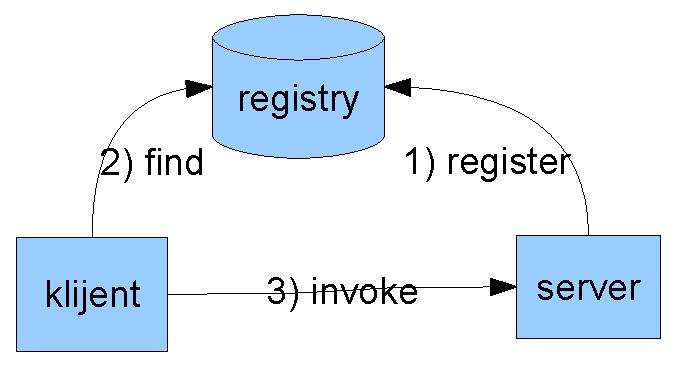
\includegraphics[width=10cm]{pic01.pdf}
  \end{center}
}
\frame{
  \frametitle{RMI klijent i server komuniciraju preko posrednika}
  \begin{center}
    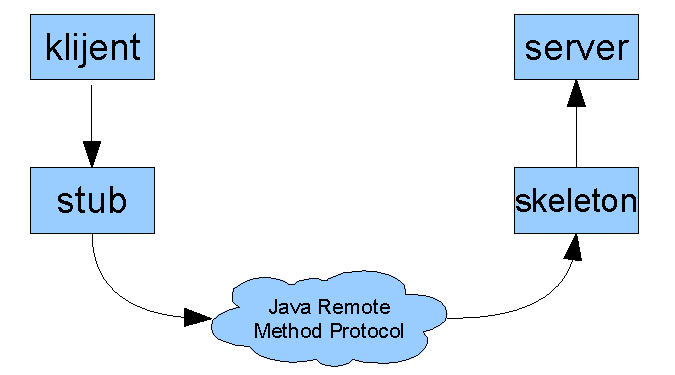
\includegraphics[width=10cm]{pic02.pdf}
  \end{center}
}
\frame{
  \frametitle{Primer elementarnog RMI klijenta i servera}
  \begin{itemize}
    \item Primer 1
  \end{itemize}
}
\frame{
  \frametitle{RMI i prenos programskog koda}
  \begin{itemize}
    \item Prilikom poziva metode RMI objekta...
    \item ...kao parametar možemo proslediti instancu klase koja nasleđuje tip parametra
    \item Tada će JVM preneti i programski kod potrebne klase!
    \item Primer 2
  \end{itemize}
}
\frame{
  \frametitle{JNDI}
  \begin{itemize}
    \item Java Naming and Directory Interface
    \item Standardni API za pristup različitim servisima imena
    \item I različitim direktorijumskim servisima
    \item Servis imena: mapira ime (string) $\leftrightarrow$ objekat
    \begin{itemize}
      \item Fajl-sistem
      \item RMI registry
    \end{itemize}
    \item Direktorijumski servis: objekti se dodatno opisuju pomoću atributa
    \begin{itemize}
      \item DNS
      \item LDAP / Active Directory / NDS...
    \end{itemize}
    \item Pristup različitim servisima obavlja se kroz isti API ali preko različitog ,,provajdera`` (tj. drajvera)
    \begin{itemize}
      \item analogno sa JDBC
    \end{itemize}
  \end{itemize}
}
\frame{
  \frametitle{JNDI}
  \begin{itemize}
    \item Primer 3
  \end{itemize}
}
\frame{
  \frametitle{RMI + JNDI}
  \begin{itemize}
    \item Umesto Naming.lookup() možemo da koristimo JNDI API za pronalaženje RMI objekta
    \item Primer 4
  \end{itemize}
}
\section{EJB3}
\frame{
\frametitle{Java EE}
\begin{itemize}
  \item Enterprise JavaBeans (EJB) 3.0 --- JSR-220
  \item JavaServer Pages (JSP) 2.1 --- JSR-245
  \item JavaServer Faces (JSF) 1.2 --- JSR-252
  \item JSP Standard Template Library (JSTL) 1.1 --- JSR-52
  \item Java API for XML Binding (JAXB) 2.0 --- JSR-222
  \item Java API for XML -- Web Services (JAX-WS) 2.0 --- JSR-224
  \item Web Service Annotations (WS Annotations) --- JSR-181
\end{itemize}
}
\frame{
  \frametitle{EJB 3.0}
  \begin{itemize}
    \item Programski model za pisanje distribuiranih komponenti
    \item Svrha komponenti:
    \begin{itemize}
      \item Vrše programsku obradu (implementiraju ,,poslovnu logiku``) --- \myblue{session beans}
      \item Reprezentuju podatke u (relacionoj) bazi podataka --- \\ \myblue{entities}
      \item Vrše programsku obradu uz asinhrono pozivanje --- \myblue{message-driven beans} 
    \end{itemize}
    \item Distribuirane: dostupne preko mreže
  \end{itemize}
}
\frame{
  \frametitle{EJB 3.0}
  \begin{itemize}
    \item Temeljno prerađena specifikacija bazirana na prethodnim iskustvima
    \item Loša iskustva sa EJB 2.1
    \item Dobra iskustva iz različitih (open source) projekata
    \begin{itemize}
      \item Hibernate: O/R mapiranje ,,urađeno kako treba``
      \item Spring: životni ciklus, dependency injection, AOP
    \end{itemize}
    \item upotreba \myblue{anotacija} eliminiše XML konfiguracione fajlove
  \end{itemize}
}
\section{Session beans}
\frame{
  \frametitle{EJB 3.0: Session bean}
  \begin{itemize}
    \item Session bean se sastoji iz
    \begin{itemize}
      \item remote i/ili lokalnog interfejsa
      \item bean klase
    \end{itemize}
    \item Klijent ga pronalazi pomoću JNDI-a
    \item i poziva njegove metode
  \end{itemize}
}
\frame{
  \frametitle{Dve vrste session beanova}
  \begin{itemize}
    \item \myblue{Stateless}: ne pamti stanje između poziva svojih metoda
    \begin{itemize}
      \item bean klasa može imati atribute ali se ne garantuje za njihov sadržaj prilikom sledećeg poziva!
    \end{itemize}
    \item \myblue{Stateful}: pamti stanje između poziva
  \end{itemize}
}
\frame{
  \frametitle{Stateless session bean}
  \begin{itemize}
    \item Primer 5
  \end{itemize}
}
\frame{
  \frametitle{Stateful session bean}
  \begin{itemize}
    \item Primer 6
  \end{itemize}
}
\frame{
  \frametitle{Stateless vs stateful: performanse}
  \begin{itemize}
    \item Stateless
    \begin{itemize}
      \item jednostavni za pooling, zaključavanje na nivou poziva metode
    \end{itemize}
    \item Stateful
    \begin{itemize}
      \item komplikovani za pooling, zaključavanje na nivou celog objekta
    \end{itemize}
  \end{itemize}
}
\frame{
  \frametitle{Životni ciklus session beana}
  \begin{center}
    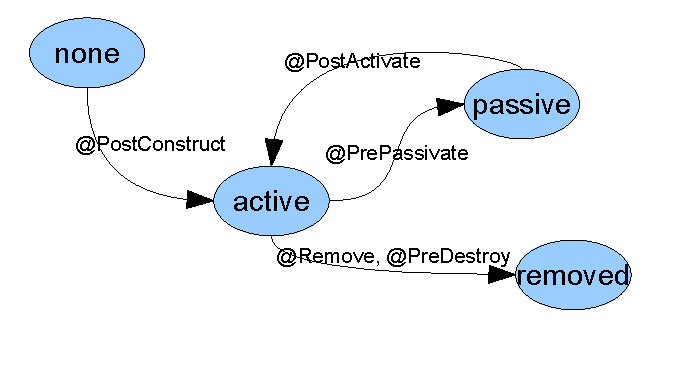
\includegraphics[width=10cm]{pic03.pdf}
  \end{center}
  \begin{itemize}
    \item Primer 7
  \end{itemize}
}
\frame{
  \frametitle{Session bean poziva drugi session bean}
  \begin{itemize}
    \item Prvi SB se ponaša kao klijent za drugi SB
    \item Ako se nalaze u istom kontejneru, može da koristi lokalni interfejs
    \item Pronalazi ga preko JNDI konteksta
    \item Inicijalni kontekst se konstruiše bez parametara
    \item Primer 8
  \end{itemize}
}
\section[DI]{Dependency injection}
\frame{
  \frametitle{Session bean i dependency injection}
  \begin{itemize}
    \item Drugi način da jedan SB dobije referencu na drugi je pomoću \myblue{dependency injection} mehanizma
    \item Referencu na drugi SB upisuje {\bf kontejner} u atribut prvog SB
    \item Atribut je potrebno označiti anotacijom {\bf @EJB}
    \item Primer 9
  \end{itemize}
}
\frame{
  \frametitle{Session bean i dependency injection}
  \begin{itemize}
    \item Dependency injection je moguć u sledećim slučajevima \\ (bean A $\rightarrow$ (poziva) bean B)
    \begin{itemize}
      \item stateless $\rightarrow$ stateless
      \item stateful $\rightarrow$ stateless
      \item stateful $\rightarrow$ stateful
    \end{itemize}
    \item A zabranjen je u slučaju
    \begin{itemize}
      \item stateless $\rightarrow$ stateful
    \end{itemize}
  \end{itemize}
}
\frame{
  \frametitle{Session bean i dependency injection}
  \begin{itemize}
    \item Anotacijom {\bf @Resource} mogu da se označe atributi sledećeg tipa
    \begin{itemize}
      \item javax.ejb.SessionContext
      \item javax.sql.DataSource
      \item javax.transaction.UserTransaction
      \item javax.jms.Queue, javax.jms.Topic
      \item \ldots
    \end{itemize}
    \item Anotacijom {\bf @PersistenceContext} označava se atribut tipa
    \begin{itemize}
      \item javax.persistence.EntityManager
    \end{itemize}
    \item Anotacijom {\bf @PersistenceContextFactory} označava se atribut tipa
    \begin{itemize}
      \item javax.persistence.EntityManagerFactory
    \end{itemize}
  \end{itemize}
}
\section[AOP]{Elementi aspekt-orijentisanog programiranja}
\frame{
  \frametitle{Aspekt-orijentisano programiranje (AOP)}
  \begin{itemize}
    \item Sredstvo za izražavanje određenih pravila/procedura koja se mogu primeniti na više mesta u programu
    \item Npr. logovanje, kontrola pristupa, \ldots -- aspekti programa koji nisu direktno vezani za poslovnu logiku
      i često izgledaju isto za različite poslovne procedure
    \item \myblue{Aspekt} je parče koda koji se može vezati za neku metodu tako da se izvrši
    \begin{itemize}
      \item pre poziva metode
      \item posle poziva metode
      \item oko poziva metode (obuhvata poziv)
    \end{itemize}
  \end{itemize}
}
\frame{
  \frametitle{Session beans i AOP}
  \begin{itemize}
    \item U EJB 3.0 aspekti mogu da {\bf obuhvate} poziv metode
    \item Metodu je potrebno označiti anotacijom {\bf @Interceptor}
    \item Ako ima više aspekata onda {\bf @Interceptors}
    \item Parametar ove anotacije je klasa koja sadrži aspekt
    \item Aspekt je metoda u klasi označena anotacijom {\bf @AroundInvoke}
    \item Primer 10
  \end{itemize}
}
\frame{
  \frametitle{Interceptori i životni ciklus beana}
  \begin{itemize}
    \item Klasa navedena kao @Interceptor može sadržati i metode za obaveštavanje o događajima u životnom ciklusu
    \item U primeru 7 te metode su bile deo bean klase
    \item Možemo ih premestiti u interceptor klasu
    \item Koristimo iste anotacije: @PostConstruct, @PrePassivate, @PostActivate, @PreDestroy
    \item Primer 11
  \end{itemize}
}

\end{document}
